\documentclass[1p]{elsarticle_modified}
%\bibliographystyle{elsarticle-num}

%\usepackage[colorlinks]{hyperref}
%\usepackage{abbrmath_seonhwa} %\Abb, \Ascr, \Acal ,\Abf, \Afrak
\usepackage{amsfonts}
\usepackage{amssymb}
\usepackage{amsmath}
\usepackage{amsthm}
\usepackage{scalefnt}
\usepackage{amsbsy}
\usepackage{kotex}
\usepackage{caption}
\usepackage{subfig}
\usepackage{color}
\usepackage{graphicx}
\usepackage{xcolor} %% white, black, red, green, blue, cyan, magenta, yellow
\usepackage{float}
\usepackage{setspace}
\usepackage{hyperref}

\usepackage{tikz}
\usetikzlibrary{arrows}

\usepackage{multirow}
\usepackage{array} % fixed length table
\usepackage{hhline}

%%%%%%%%%%%%%%%%%%%%%
\makeatletter
\renewcommand*\env@matrix[1][\arraystretch]{%
	\edef\arraystretch{#1}%
	\hskip -\arraycolsep
	\let\@ifnextchar\new@ifnextchar
	\array{*\c@MaxMatrixCols c}}
\makeatother %https://tex.stackexchange.com/questions/14071/how-can-i-increase-the-line-spacing-in-a-matrix
%%%%%%%%%%%%%%%

\usepackage[normalem]{ulem}

\newcommand{\msout}[1]{\ifmmode\text{\sout{\ensuremath{#1}}}\else\sout{#1}\fi}
%SOURCE: \msout is \stkout macro in https://tex.stackexchange.com/questions/20609/strikeout-in-math-mode

\newcommand{\cancel}[1]{
	\ifmmode
	{\color{red}\msout{#1}}
	\else
	{\color{red}\sout{#1}}
	\fi
}

\newcommand{\add}[1]{
	{\color{blue}\uwave{#1}}
}

\newcommand{\replace}[2]{
	\ifmmode
	{\color{red}\msout{#1}}{\color{blue}\uwave{#2}}
	\else
	{\color{red}\sout{#1}}{\color{blue}\uwave{#2}}
	\fi
}

\newcommand{\Sol}{\mathcal{S}} %segment
\newcommand{\D}{D} %diagram
\newcommand{\A}{\mathcal{A}} %arc


%%%%%%%%%%%%%%%%%%%%%%%%%%%%%5 test

\def\sl{\operatorname{\textup{SL}}(2,\Cbb)}
\def\psl{\operatorname{\textup{PSL}}(2,\Cbb)}
\def\quan{\mkern 1mu \triangleright \mkern 1mu}

\theoremstyle{definition}
\newtheorem{thm}{Theorem}[section]
\newtheorem{prop}[thm]{Proposition}
\newtheorem{lem}[thm]{Lemma}
\newtheorem{ques}[thm]{Question}
\newtheorem{cor}[thm]{Corollary}
\newtheorem{defn}[thm]{Definition}
\newtheorem{exam}[thm]{Example}
\newtheorem{rmk}[thm]{Remark}
\newtheorem{alg}[thm]{Algorithm}

\newcommand{\I}{\sqrt{-1}}
\begin{document}

%\begin{frontmatter}
%
%\title{Boundary parabolic representations of knots up to 8 crossings}
%
%%% Group authors per affiliation:
%\author{Yunhi Cho} 
%\address{Department of Mathematics, University of Seoul, Seoul, Korea}
%\ead{yhcho@uos.ac.kr}
%
%
%\author{Seonhwa Kim} %\fnref{s_kim}}
%\address{Center for Geometry and Physics, Institute for Basic Science, Pohang, 37673, Korea}
%\ead{ryeona17@ibs.re.kr}
%
%\author{Hyuk Kim}
%\address{Department of Mathematical Sciences, Seoul National University, Seoul 08826, Korea}
%\ead{hyukkim@snu.ac.kr}
%
%\author{Seokbeom Yoon}
%\address{Department of Mathematical Sciences, Seoul National University, Seoul, 08826,  Korea}
%\ead{sbyoon15@snu.ac.kr}
%
%\begin{abstract}
%We find all boundary parabolic representation of knots up to 8 crossings.
%
%\end{abstract}
%\begin{keyword}
%    \MSC[2010] 57M25 
%\end{keyword}
%
%\end{frontmatter}

%\linenumbers
%\tableofcontents
%
\newcommand\colored[1]{\textcolor{white}{\rule[-0.35ex]{0.8em}{1.4ex}}\kern-0.8em\color{red} #1}%
%\newcommand\colored[1]{\textcolor{white}{ #1}\kern-2.17ex	\textcolor{white}{ #1}\kern-1.81ex	\textcolor{white}{ #1}\kern-2.15ex\color{red}#1	}

{\Large $\underline{12a_{0521}~(K12a_{0521})}$}

\setlength{\tabcolsep}{10pt}
\renewcommand{\arraystretch}{1.6}
\vspace{1cm}\begin{tabular}{m{100pt}>{\centering\arraybackslash}m{274pt}}
\multirow{5}{120pt}{
	\centering
	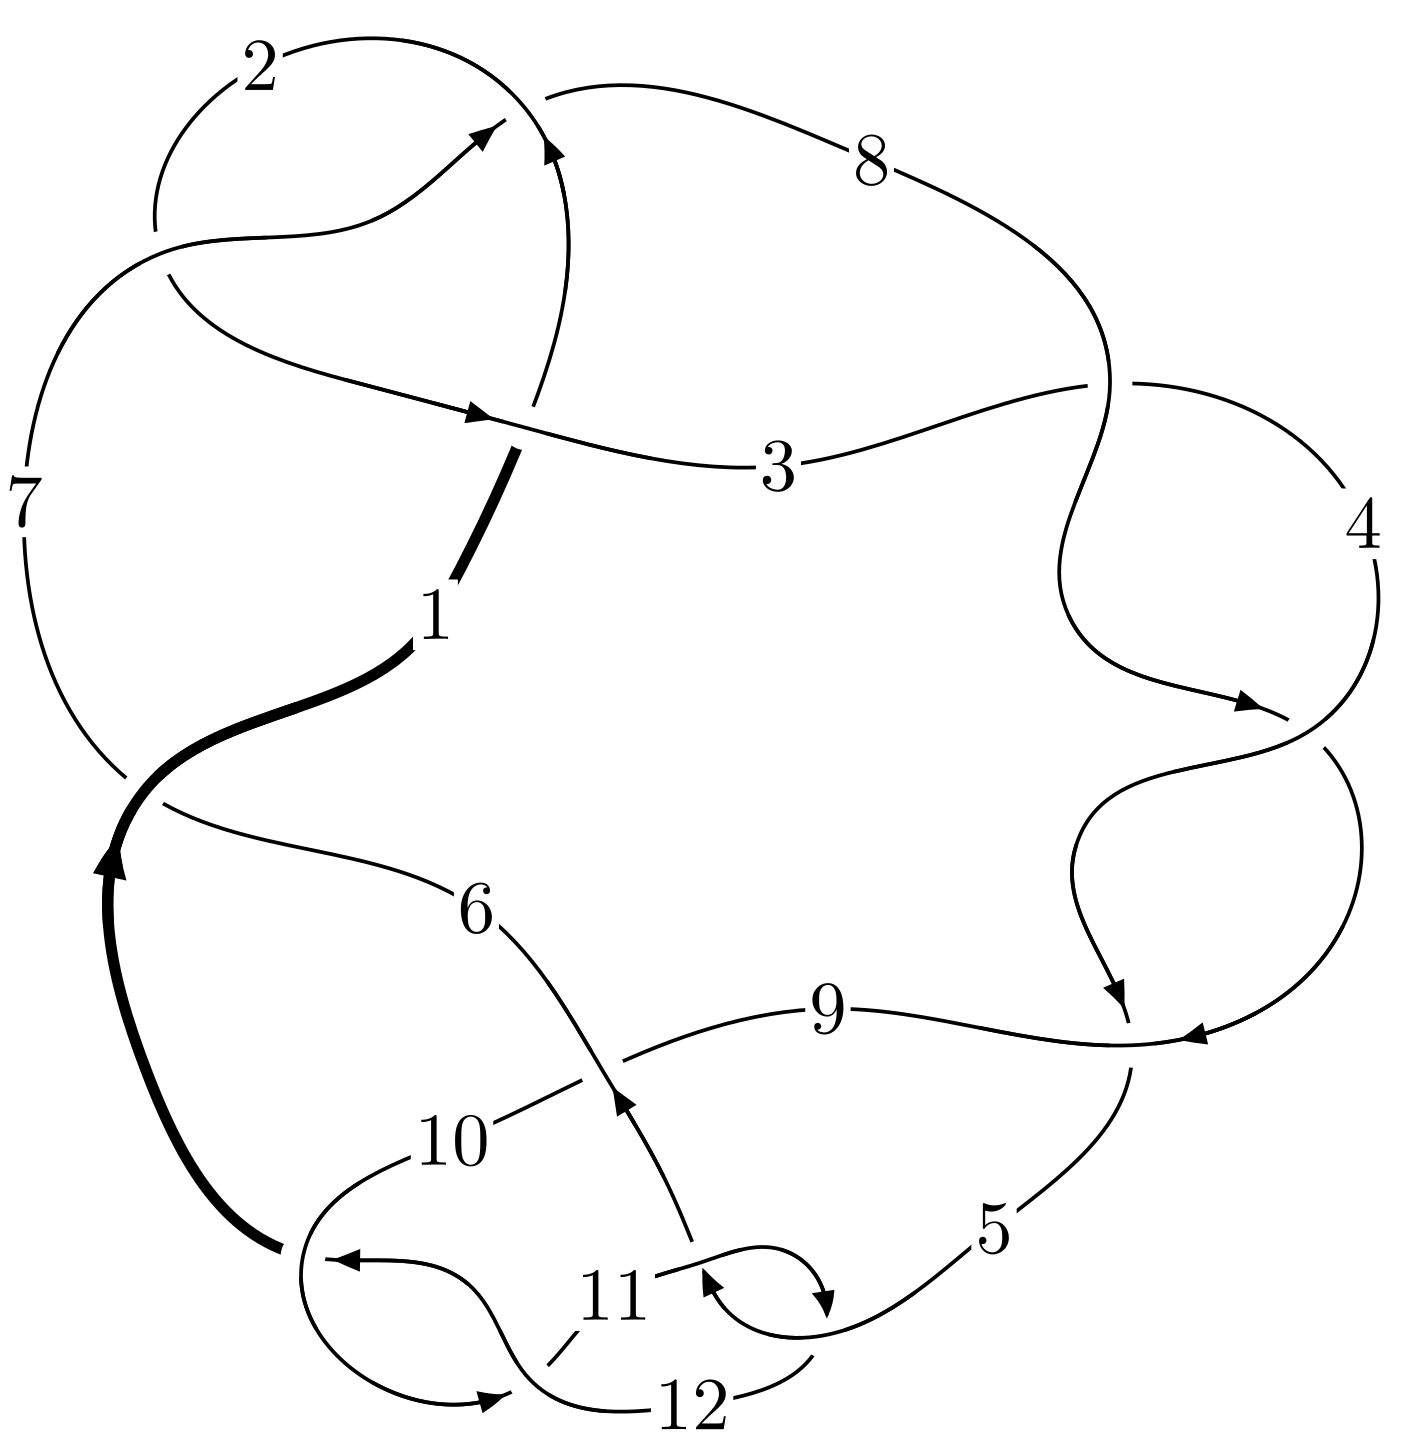
\includegraphics[width=112pt]{../../../GIT/diagram.site/Diagrams/png/1322_12a_0521.png}\\
\ \ \ A knot diagram\footnotemark}&
\allowdisplaybreaks
\textbf{Linearized knot diagam} \\
\cline{2-2}
 &
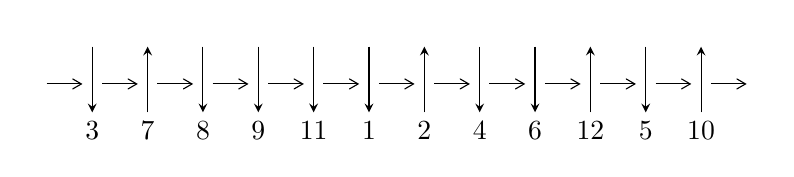
\begin{tikzpicture}[x=20pt, y=17pt]
	% nodes
	\node (C0) at (0, 0) {};
	\node (C1) at (1, 0) {};
	\node (C1U) at (1, +1) {};
	\node (C1D) at (1, -1) {3};

	\node (C2) at (2, 0) {};
	\node (C2U) at (2, +1) {};
	\node (C2D) at (2, -1) {7};

	\node (C3) at (3, 0) {};
	\node (C3U) at (3, +1) {};
	\node (C3D) at (3, -1) {8};

	\node (C4) at (4, 0) {};
	\node (C4U) at (4, +1) {};
	\node (C4D) at (4, -1) {9};

	\node (C5) at (5, 0) {};
	\node (C5U) at (5, +1) {};
	\node (C5D) at (5, -1) {11};

	\node (C6) at (6, 0) {};
	\node (C6U) at (6, +1) {};
	\node (C6D) at (6, -1) {1};

	\node (C7) at (7, 0) {};
	\node (C7U) at (7, +1) {};
	\node (C7D) at (7, -1) {2};

	\node (C8) at (8, 0) {};
	\node (C8U) at (8, +1) {};
	\node (C8D) at (8, -1) {4};

	\node (C9) at (9, 0) {};
	\node (C9U) at (9, +1) {};
	\node (C9D) at (9, -1) {6};

	\node (C10) at (10, 0) {};
	\node (C10U) at (10, +1) {};
	\node (C10D) at (10, -1) {12};

	\node (C11) at (11, 0) {};
	\node (C11U) at (11, +1) {};
	\node (C11D) at (11, -1) {5};

	\node (C12) at (12, 0) {};
	\node (C12U) at (12, +1) {};
	\node (C12D) at (12, -1) {10};
	\node (C13) at (13, 0) {};

	% arrows
	\draw[->,>={angle 60}]
	(C0) edge (C1) (C1) edge (C2) (C2) edge (C3) (C3) edge (C4) (C4) edge (C5) (C5) edge (C6) (C6) edge (C7) (C7) edge (C8) (C8) edge (C9) (C9) edge (C10) (C10) edge (C11) (C11) edge (C12) (C12) edge (C13) ;	\draw[->,>=stealth]
	(C1U) edge (C1D) (C2D) edge (C2U) (C3U) edge (C3D) (C4U) edge (C4D) (C5U) edge (C5D) (C6U) edge (C6D) (C7D) edge (C7U) (C8U) edge (C8D) (C9U) edge (C9D) (C10D) edge (C10U) (C11U) edge (C11D) (C12D) edge (C12U) ;
	\end{tikzpicture} \\
\hhline{~~} \\& 
\textbf{Solving Sequence} \\ \cline{2-2} 
 &
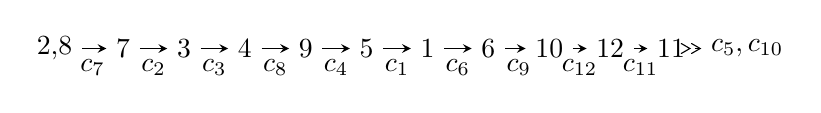
\begin{tikzpicture}[x=22pt, y=7pt]
	% node
	\node (A0) at (-1/8, 0) {2,8};
	\node (A1) at (1, 0) {7};
	\node (A2) at (2, 0) {3};
	\node (A3) at (3, 0) {4};
	\node (A4) at (4, 0) {9};
	\node (A5) at (5, 0) {5};
	\node (A6) at (6, 0) {1};
	\node (A7) at (7, 0) {6};
	\node (A8) at (8, 0) {10};
	\node (A9) at (9, 0) {12};
	\node (A10) at (10, 0) {11};
	\node (C1) at (1/2, -1) {$c_{7}$};
	\node (C2) at (3/2, -1) {$c_{2}$};
	\node (C3) at (5/2, -1) {$c_{3}$};
	\node (C4) at (7/2, -1) {$c_{8}$};
	\node (C5) at (9/2, -1) {$c_{4}$};
	\node (C6) at (11/2, -1) {$c_{1}$};
	\node (C7) at (13/2, -1) {$c_{6}$};
	\node (C8) at (15/2, -1) {$c_{9}$};
	\node (C9) at (17/2, -1) {$c_{12}$};
	\node (C10) at (19/2, -1) {$c_{11}$};
	\node (A11) at (45/4, 0) {$c_{5},c_{10}$};

	% edge
	\draw[->,>=stealth]	
	(A0) edge (A1) (A1) edge (A2) (A2) edge (A3) (A3) edge (A4) (A4) edge (A5) (A5) edge (A6) (A6) edge (A7) (A7) edge (A8) (A8) edge (A9) (A9) edge (A10) ;
	\draw[->>,>={angle 60}]	
	(A10) edge (A11);
\end{tikzpicture} \\ 

\end{tabular} \\

\footnotetext{
The image of knot diagram is generated by the software ``\textbf{Draw programme}" developed by Andrew Bartholomew(\url{http://www.layer8.co.uk/maths/draw/index.htm\#Running-draw}), where we modified some parts for our purpose(\url{https://github.com/CATsTAILs/LinksPainter}).
}\phantom \\ \newline 
\centering \textbf{Ideals for irreducible components\footnotemark of $X_{\text{par}}$} 
 
\begin{align*}
I^u_{1}&=\langle 
u^{56}- u^{55}+\cdots+2 u^3-1\rangle \\
\\
\end{align*}
\raggedright * 1 irreducible components of $\dim_{\mathbb{C}}=0$, with total 56 representations.\\
\footnotetext{All coefficients of polynomials are rational numbers. But the coefficients are sometimes approximated in decimal forms when there is not enough margin.}
\newpage
\renewcommand{\arraystretch}{1}
\centering \section*{I. $I^u_{1}= \langle u^{56}- u^{55}+\cdots+2 u^3-1 \rangle$}
\flushleft \textbf{(i) Arc colorings}\\
\begin{tabular}{m{7pt} m{180pt} m{7pt} m{180pt} }
\flushright $a_{2}=$&$\begin{pmatrix}0\\u\end{pmatrix}$ \\
\flushright $a_{8}=$&$\begin{pmatrix}1\\0\end{pmatrix}$ \\
\flushright $a_{7}=$&$\begin{pmatrix}1\\u^2\end{pmatrix}$ \\
\flushright $a_{3}=$&$\begin{pmatrix}u\\u^3+u\end{pmatrix}$ \\
\flushright $a_{4}=$&$\begin{pmatrix}- u^3\\u^3+u\end{pmatrix}$ \\
\flushright $a_{9}=$&$\begin{pmatrix}- u^6- u^4+1\\u^6+2 u^4+u^2\end{pmatrix}$ \\
\flushright $a_{5}=$&$\begin{pmatrix}u^9+2 u^7+u^5-2 u^3- u\\- u^9-3 u^7-3 u^5+u\end{pmatrix}$ \\
\flushright $a_{1}=$&$\begin{pmatrix}u^3\\u^5+u^3+u\end{pmatrix}$ \\
\flushright $a_{6}=$&$\begin{pmatrix}- u^6- u^4+1\\- u^8-2 u^6-2 u^4\end{pmatrix}$ \\
\flushright $a_{10}=$&$\begin{pmatrix}- u^{20}-5 u^{18}-11 u^{16}-10 u^{14}+2 u^{12}+13 u^{10}+9 u^8-2 u^6-5 u^4- u^2+1\\- u^{22}-6 u^{20}-17 u^{18}-26 u^{16}-20 u^{14}+13 u^{10}+10 u^8+3 u^6+2 u^4+u^2\end{pmatrix}$ \\
\flushright $a_{12}=$&$\begin{pmatrix}u^{37}+10 u^{35}+\cdots+2 u^3- u\\u^{39}+11 u^{37}+\cdots- u^5+u\end{pmatrix}$ \\
\flushright $a_{11}=$&$\begin{pmatrix}- u^{54}-15 u^{52}+\cdots-7 u^4+1\\- u^{55}+u^{54}+\cdots+2 u^3-1\end{pmatrix}$\\&\end{tabular}
\flushleft \textbf{(ii) Obstruction class $= -1$}\\~\\
\flushleft \textbf{(iii) Cusp Shapes $= 4 u^{54}-4 u^{53}+\cdots-4 u-6$}\\~\\
\newpage\renewcommand{\arraystretch}{1}
\flushleft \textbf{(iv) u-Polynomials at the component}\newline \\
\begin{tabular}{m{50pt}|m{274pt}}
Crossings & \hspace{64pt}u-Polynomials at each crossing \\
\hline $$\begin{aligned}c_{1}\end{aligned}$$&$\begin{aligned}
&u^{56}+33 u^{55}+\cdots-10 u^2+1
\end{aligned}$\\
\hline $$\begin{aligned}c_{2},c_{7}\end{aligned}$$&$\begin{aligned}
&u^{56}+u^{55}+\cdots-2 u^3-1
\end{aligned}$\\
\hline $$\begin{aligned}c_{3},c_{4},c_{6}\\c_{8}\end{aligned}$$&$\begin{aligned}
&u^{56}- u^{55}+\cdots-14 u-1
\end{aligned}$\\
\hline $$\begin{aligned}c_{5},c_{11}\end{aligned}$$&$\begin{aligned}
&u^{56}- u^{55}+\cdots-2 u-1
\end{aligned}$\\
\hline $$\begin{aligned}c_{9}\end{aligned}$$&$\begin{aligned}
&u^{56}+5 u^{55}+\cdots-4088 u-1767
\end{aligned}$\\
\hline $$\begin{aligned}c_{10},c_{12}\end{aligned}$$&$\begin{aligned}
&u^{56}-17 u^{55}+\cdots+10 u^2+1
\end{aligned}$\\
\hline
\end{tabular}\\~\\
\newpage\renewcommand{\arraystretch}{1}
\flushleft \textbf{(v) Riley Polynomials at the component}\newline \\
\begin{tabular}{m{50pt}|m{274pt}}
Crossings & \hspace{64pt}Riley Polynomials at each crossing \\
\hline $$\begin{aligned}c_{1}\end{aligned}$$&$\begin{aligned}
&y^{56}-19 y^{55}+\cdots-20 y+1
\end{aligned}$\\
\hline $$\begin{aligned}c_{2},c_{7}\end{aligned}$$&$\begin{aligned}
&y^{56}+33 y^{55}+\cdots-10 y^2+1
\end{aligned}$\\
\hline $$\begin{aligned}c_{3},c_{4},c_{6}\\c_{8}\end{aligned}$$&$\begin{aligned}
&y^{56}-71 y^{55}+\cdots+96 y+1
\end{aligned}$\\
\hline $$\begin{aligned}c_{5},c_{11}\end{aligned}$$&$\begin{aligned}
&y^{56}+17 y^{55}+\cdots+10 y^2+1
\end{aligned}$\\
\hline $$\begin{aligned}c_{9}\end{aligned}$$&$\begin{aligned}
&y^{56}-27 y^{55}+\cdots-19630828 y+3122289
\end{aligned}$\\
\hline $$\begin{aligned}c_{10},c_{12}\end{aligned}$$&$\begin{aligned}
&y^{56}+45 y^{55}+\cdots+20 y+1
\end{aligned}$\\
\hline
\end{tabular}\\~\\
\newpage\flushleft \textbf{(vi) Complex Volumes and Cusp Shapes}
$$\begin{array}{c|c|c}  
\text{Solutions to }I^u_{1}& \I (\text{vol} + \sqrt{-1}CS) & \text{Cusp shape}\\
 \hline 
\begin{aligned}
u &= -0.405867 + 0.888923 I\end{aligned}
 & -1.83499 - 1.34944 I & -6.35701 + 4.05456 I \\ \hline\begin{aligned}
u &= -0.405867 - 0.888923 I\end{aligned}
 & -1.83499 + 1.34944 I & -6.35701 - 4.05456 I \\ \hline\begin{aligned}
u &= -0.021918 + 1.036680 I\end{aligned}
 & -4.65561 - 2.80215 I & -13.44960 + 3.08888 I \\ \hline\begin{aligned}
u &= -0.021918 - 1.036680 I\end{aligned}
 & -4.65561 + 2.80215 I & -13.44960 - 3.08888 I \\ \hline\begin{aligned}
u &= \phantom{-}0.437414 + 0.848600 I\end{aligned}
 & -1.27504 + 6.58005 I & -4.46879 - 9.66669 I \\ \hline\begin{aligned}
u &= \phantom{-}0.437414 - 0.848600 I\end{aligned}
 & -1.27504 - 6.58005 I & -4.46879 + 9.66669 I \\ \hline\begin{aligned}
u &= -0.917081 + 0.022864 I\end{aligned}
 & -13.20330 + 2.37614 I & -9.77936 - 0.20355 I \\ \hline\begin{aligned}
u &= -0.917081 - 0.022864 I\end{aligned}
 & -13.20330 - 2.37614 I & -9.77936 + 0.20355 I \\ \hline\begin{aligned}
u &= \phantom{-}0.915655 + 0.028828 I\end{aligned}
 & -12.4108 - 8.4052 I & -8.44929 + 5.11391 I \\ \hline\begin{aligned}
u &= \phantom{-}0.915655 - 0.028828 I\end{aligned}
 & -12.4108 + 8.4052 I & -8.44929 - 5.11391 I \\ \hline\begin{aligned}
u &= -0.307186 + 1.049610 I\end{aligned}
 & -1.50462 - 0.72055 I & -7.04900 + 0. I\phantom{ +0.000000I} \\ \hline\begin{aligned}
u &= -0.307186 - 1.049610 I\end{aligned}
 & -1.50462 + 0.72055 I & -7.04900 + 0. I\phantom{ +0.000000I} \\ \hline\begin{aligned}
u &= -0.904607\phantom{ +0.000000I}\end{aligned}
 & -9.25956\phantom{ +0.000000I} & -9.91870\phantom{ +0.000000I} \\ \hline\begin{aligned}
u &= \phantom{-}0.894317 + 0.015919 I\end{aligned}
 & -5.91089 - 3.18842 I & -3.80019 + 3.52000 I \\ \hline\begin{aligned}
u &= \phantom{-}0.894317 - 0.015919 I\end{aligned}
 & -5.91089 + 3.18842 I & -3.80019 - 3.52000 I \\ \hline\begin{aligned}
u &= -0.435609 + 1.059800 I\end{aligned}
 & -0.58121 - 5.72992 I & -4.00000 + 8.34586 I \\ \hline\begin{aligned}
u &= -0.435609 - 1.059800 I\end{aligned}
 & -0.58121 + 5.72992 I & -4.00000 - 8.34586 I \\ \hline\begin{aligned}
u &= \phantom{-}0.386574 + 1.089770 I\end{aligned}
 & -3.86140 + 3.45773 I & -12.70884 - 4.98853 I \\ \hline\begin{aligned}
u &= \phantom{-}0.386574 - 1.089770 I\end{aligned}
 & -3.86140 - 3.45773 I & -12.70884 + 4.98853 I \\ \hline\begin{aligned}
u &= \phantom{-}0.398205 + 0.739047 I\end{aligned}
 & \phantom{-}2.87979 + 1.78352 I & \phantom{-}2.98966 - 4.90547 I \\ \hline\begin{aligned}
u &= \phantom{-}0.398205 - 0.739047 I\end{aligned}
 & \phantom{-}2.87979 - 1.78352 I & \phantom{-}2.98966 + 4.90547 I \\ \hline\begin{aligned}
u &= -0.196934 + 0.792679 I\end{aligned}
 & -0.547592 - 1.072840 I & -7.44811 + 6.01442 I \\ \hline\begin{aligned}
u &= -0.196934 - 0.792679 I\end{aligned}
 & -0.547592 + 1.072840 I & -7.44811 - 6.01442 I \\ \hline\begin{aligned}
u &= -0.305708 + 1.152470 I\end{aligned}
 & -7.27525 + 3.27832 I & \phantom{-0.000000 } 0 \\ \hline\begin{aligned}
u &= -0.305708 - 1.152470 I\end{aligned}
 & -7.27525 - 3.27832 I & \phantom{-0.000000 } 0 \\ \hline\begin{aligned}
u &= \phantom{-}0.325359 + 1.152680 I\end{aligned}
 & -7.79706 + 2.53101 I & \phantom{-0.000000 } 0 \\ \hline\begin{aligned}
u &= \phantom{-}0.325359 - 1.152680 I\end{aligned}
 & -7.79706 - 2.53101 I & \phantom{-0.000000 } 0 \\ \hline\begin{aligned}
u &= -0.466232 + 1.103460 I\end{aligned}
 & -6.06698 - 10.74040 I & \phantom{-0.000000 } 0 \\ \hline\begin{aligned}
u &= -0.466232 - 1.103460 I\end{aligned}
 & -6.06698 + 10.74040 I & \phantom{-0.000000 } 0 \\ \hline\begin{aligned}
u &= \phantom{-}0.453460 + 1.112820 I\end{aligned}
 & -6.83086 + 5.00850 I & \phantom{-0.000000 } 0\\
 \hline 
 \end{array}$$\newpage$$\begin{array}{c|c|c}  
\text{Solutions to }I^u_{1}& \I (\text{vol} + \sqrt{-1}CS) & \text{Cusp shape}\\
 \hline 
\begin{aligned}
u &= \phantom{-}0.453460 - 1.112820 I\end{aligned}
 & -6.83086 - 5.00850 I & \phantom{-0.000000 } 0 \\ \hline\begin{aligned}
u &= \phantom{-}0.421866 + 0.566053 I\end{aligned}
 & -0.52914 - 2.83643 I & -2.00972 + 2.39215 I \\ \hline\begin{aligned}
u &= \phantom{-}0.421866 - 0.566053 I\end{aligned}
 & -0.52914 + 2.83643 I & -2.00972 - 2.39215 I \\ \hline\begin{aligned}
u &= -0.661353 + 0.178127 I\end{aligned}
 & -3.45247 + 6.47746 I & -6.46031 - 6.34159 I \\ \hline\begin{aligned}
u &= -0.661353 - 0.178127 I\end{aligned}
 & -3.45247 - 6.47746 I & -6.46031 + 6.34159 I \\ \hline\begin{aligned}
u &= \phantom{-}0.662306 + 0.142602 I\end{aligned}
 & -4.09011 - 0.81649 I & -8.10360 + 0.92141 I \\ \hline\begin{aligned}
u &= \phantom{-}0.662306 - 0.142602 I\end{aligned}
 & -4.09011 + 0.81649 I & -8.10360 - 0.92141 I \\ \hline\begin{aligned}
u &= \phantom{-}0.460898 + 1.264040 I\end{aligned}
 & -9.81343 + 1.61572 I & \phantom{-0.000000 } 0 \\ \hline\begin{aligned}
u &= \phantom{-}0.460898 - 1.264040 I\end{aligned}
 & -9.81343 - 1.61572 I & \phantom{-0.000000 } 0 \\ \hline\begin{aligned}
u &= \phantom{-}0.477987 + 1.259180 I\end{aligned}
 & -9.68771 + 8.08384 I & \phantom{-0.000000 } 0 \\ \hline\begin{aligned}
u &= \phantom{-}0.477987 - 1.259180 I\end{aligned}
 & -9.68771 - 8.08384 I & \phantom{-0.000000 } 0 \\ \hline\begin{aligned}
u &= -0.471428 + 1.267380 I\end{aligned}
 & -13.12820 - 4.89278 I & \phantom{-0.000000 } 0 \\ \hline\begin{aligned}
u &= -0.471428 - 1.267380 I\end{aligned}
 & -13.12820 + 4.89278 I & \phantom{-0.000000 } 0 \\ \hline\begin{aligned}
u &= \phantom{-}0.456440 + 1.279200 I\end{aligned}
 & -16.4343 - 3.5507 I & \phantom{-0.000000 } 0 \\ \hline\begin{aligned}
u &= \phantom{-}0.456440 - 1.279200 I\end{aligned}
 & -16.4343 + 3.5507 I & \phantom{-0.000000 } 0 \\ \hline\begin{aligned}
u &= \phantom{-}0.489034 + 1.267150 I\end{aligned}
 & -16.1895 + 13.4198 I & \phantom{-0.000000 } 0 \\ \hline\begin{aligned}
u &= \phantom{-}0.489034 - 1.267150 I\end{aligned}
 & -16.1895 - 13.4198 I & \phantom{-0.000000 } 0 \\ \hline\begin{aligned}
u &= -0.486244 + 1.269270 I\end{aligned}
 & -17.0105 - 7.3815 I & \phantom{-0.000000 } 0 \\ \hline\begin{aligned}
u &= -0.486244 - 1.269270 I\end{aligned}
 & -17.0105 + 7.3815 I & \phantom{-0.000000 } 0 \\ \hline\begin{aligned}
u &= -0.460358 + 1.278950 I\end{aligned}
 & -17.2053 - 2.5025 I & \phantom{-0.000000 } 0 \\ \hline\begin{aligned}
u &= -0.460358 - 1.278950 I\end{aligned}
 & -17.2053 + 2.5025 I & \phantom{-0.000000 } 0 \\ \hline\begin{aligned}
u &= -0.418964 + 0.467128 I\end{aligned}
 & -0.73474 - 2.24620 I & -2.43482 + 3.10244 I \\ \hline\begin{aligned}
u &= -0.418964 - 0.467128 I\end{aligned}
 & -0.73474 + 2.24620 I & -2.43482 - 3.10244 I \\ \hline\begin{aligned}
u &= -0.530935 + 0.216533 I\end{aligned}
 & \phantom{-}1.71161 + 1.86206 I & \phantom{-}0.40956 - 4.60344 I \\ \hline\begin{aligned}
u &= -0.530935 - 0.216533 I\end{aligned}
 & \phantom{-}1.71161 - 1.86206 I & \phantom{-}0.40956 + 4.60344 I \\ \hline\begin{aligned}
u &= \phantom{-}0.517215\phantom{ +0.000000I}\end{aligned}
 & -1.03672\phantom{ +0.000000I} & -9.70580\phantom{ +0.000000I}\\
 \hline 
 \end{array}$$\newpage
\newpage\renewcommand{\arraystretch}{1}
\centering \section*{ II. u-Polynomials}
\begin{tabular}{m{50pt}|m{274pt}}
Crossings & \hspace{64pt}u-Polynomials at each crossing \\
\hline $$\begin{aligned}c_{1}\end{aligned}$$&$\begin{aligned}
&u^{56}+33 u^{55}+\cdots-10 u^2+1
\end{aligned}$\\
\hline $$\begin{aligned}c_{2},c_{7}\end{aligned}$$&$\begin{aligned}
&u^{56}+u^{55}+\cdots-2 u^3-1
\end{aligned}$\\
\hline $$\begin{aligned}c_{3},c_{4},c_{6}\\c_{8}\end{aligned}$$&$\begin{aligned}
&u^{56}- u^{55}+\cdots-14 u-1
\end{aligned}$\\
\hline $$\begin{aligned}c_{5},c_{11}\end{aligned}$$&$\begin{aligned}
&u^{56}- u^{55}+\cdots-2 u-1
\end{aligned}$\\
\hline $$\begin{aligned}c_{9}\end{aligned}$$&$\begin{aligned}
&u^{56}+5 u^{55}+\cdots-4088 u-1767
\end{aligned}$\\
\hline $$\begin{aligned}c_{10},c_{12}\end{aligned}$$&$\begin{aligned}
&u^{56}-17 u^{55}+\cdots+10 u^2+1
\end{aligned}$\\
\hline
\end{tabular}\newpage\renewcommand{\arraystretch}{1}
\centering \section*{ III. Riley Polynomials}
\begin{tabular}{m{50pt}|m{274pt}}
Crossings & \hspace{64pt}Riley Polynomials at each crossing \\
\hline $$\begin{aligned}c_{1}\end{aligned}$$&$\begin{aligned}
&y^{56}-19 y^{55}+\cdots-20 y+1
\end{aligned}$\\
\hline $$\begin{aligned}c_{2},c_{7}\end{aligned}$$&$\begin{aligned}
&y^{56}+33 y^{55}+\cdots-10 y^2+1
\end{aligned}$\\
\hline $$\begin{aligned}c_{3},c_{4},c_{6}\\c_{8}\end{aligned}$$&$\begin{aligned}
&y^{56}-71 y^{55}+\cdots+96 y+1
\end{aligned}$\\
\hline $$\begin{aligned}c_{5},c_{11}\end{aligned}$$&$\begin{aligned}
&y^{56}+17 y^{55}+\cdots+10 y^2+1
\end{aligned}$\\
\hline $$\begin{aligned}c_{9}\end{aligned}$$&$\begin{aligned}
&y^{56}-27 y^{55}+\cdots-19630828 y+3122289
\end{aligned}$\\
\hline $$\begin{aligned}c_{10},c_{12}\end{aligned}$$&$\begin{aligned}
&y^{56}+45 y^{55}+\cdots+20 y+1
\end{aligned}$\\
\hline
\end{tabular}
\vskip 2pc
\end{document}